\label{appendices}

\chapter{Commands used to run NOBLE Coder}
\label{app:commands_run_noble}

\begin{lstlisting}[language=bash]
$ java -jar NobleCoder-1.0.jar -terminology radlex \
-input [portuguese reports path] -output [output path] \
-search all-match\textit{

$ java -jar NobleCoder-1.0.jar -terminology radlex \
-input [portuguese reports path] -output [output path] \
-search best-match
\end{lstlisting}

\chapter{Uploading RadLex ontology to NOBLE}
\label{app:change_radlex_noble}

I had to edit the RadLex ontology .owl file before it could be correctly processed and uploaded to NOBLE Coder. In the original .owl file the properties  "Preferred\_name" and "Synonym" are considered to be \textit{DatatypeProperty} but I had to change both to \textit{AnnotationProperty}. That is, where in the file was

\begin{lstlisting}[language=xml]
<owl:DatatypeProperty rdf:ID="Preferred_name">
</owl:DatatypeProperty>
\end{lstlisting}

I've had to change it to:

\begin{lstlisting}[language=xml]
<owl:AnnotationProperty rdf:ID="Preferred_name">
</owl:AnnotationProperty>
\end{lstlisting}

And the analogous thing for the "Synonym" property.


\chapter{Macro Evaluations}
\label{app:macro_evaluations}

\begin{figure}[ht]
	\centering
	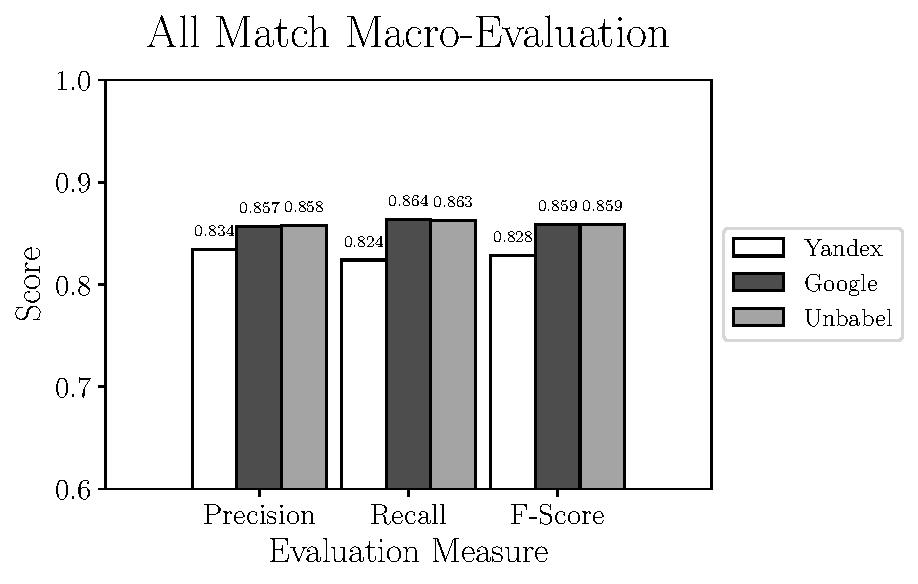
\includegraphics[width=0.9\textwidth]{SupportFiles/plots/all_match_macro_total_plot.pdf}
	\caption{Macro Evaluation of Translations being tested (All Match)}
	\label{app:macro_eval_all}
\end{figure}

\begin{figure}[ht]
	\centering
	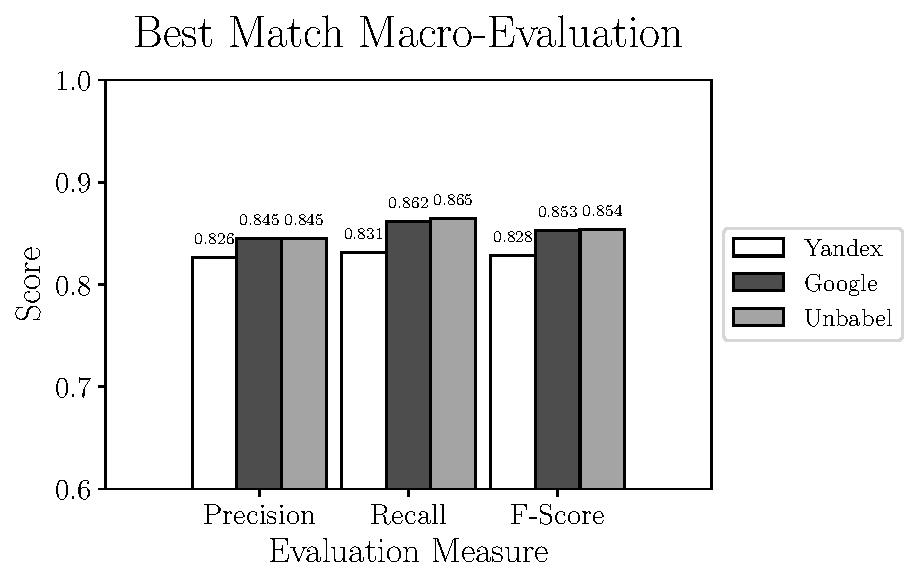
\includegraphics[width=0.9\textwidth]{SupportFiles/plots/best_match_macro_total_plot.pdf}
	\caption{Macro Evaluation of Translations being tested (Best Match)}
	\label{app:macro_eval_best}
\end{figure}

\begin{figure}[ht]
	\centering
	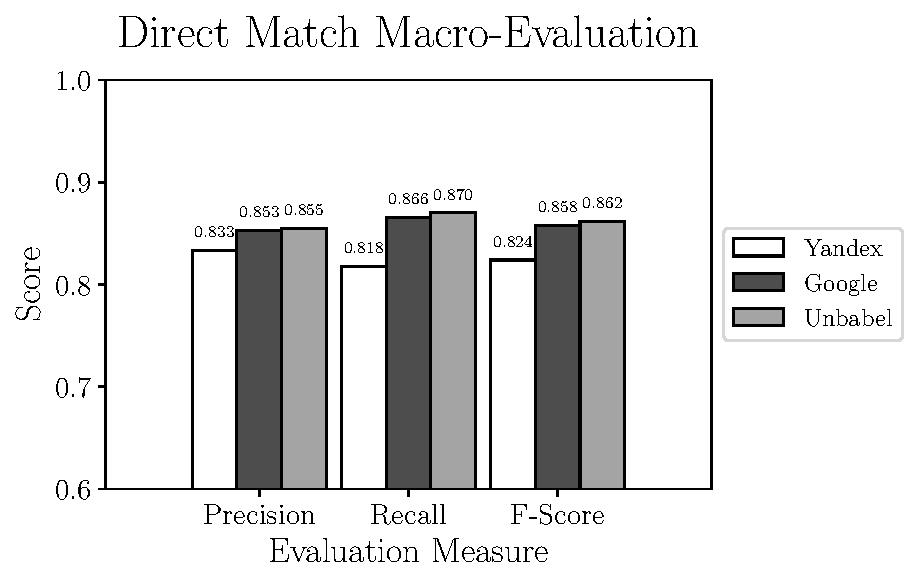
\includegraphics[width=0.9\textwidth]{SupportFiles/plots/direct_match_macro_total_plot.pdf}
	\caption{Macro Evaluation of Translations being tested (Direct Match)}
	\label{app:macro_eval_direct}
\end{figure}


\begin{figure}[ht]
	\centering
	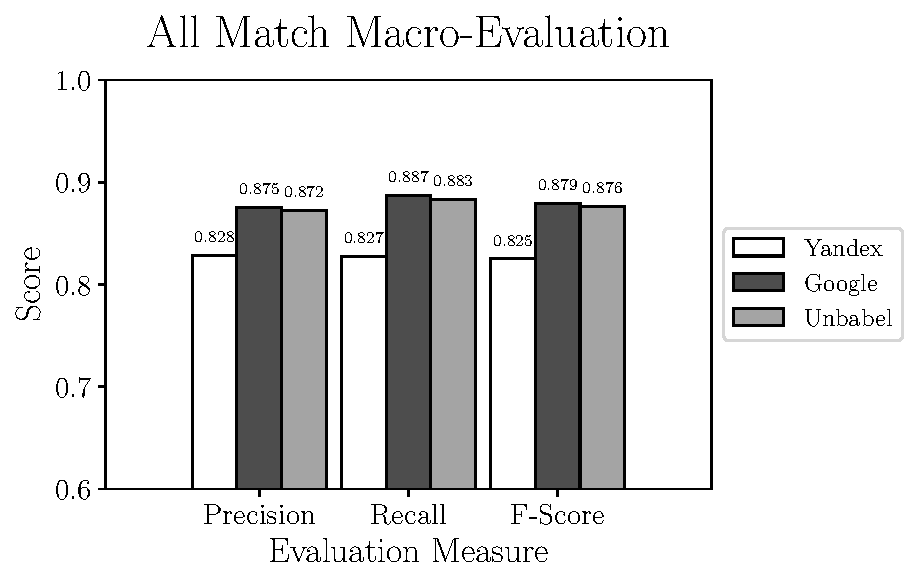
\includegraphics[width=0.9\textwidth]{SupportFiles/plots/all_match_macro_clinical_anatomical_subtrees_plot.pdf}
	\caption{Macro Evaluation of translations being tested, considering just the terms from RadLex \textit{clinical finding} and \textit{anatomical entity} subtrees (All Match)}
	\label{app:macro_eval_subtrees_all}
\end{figure}


\begin{figure}[ht]
	\centering
	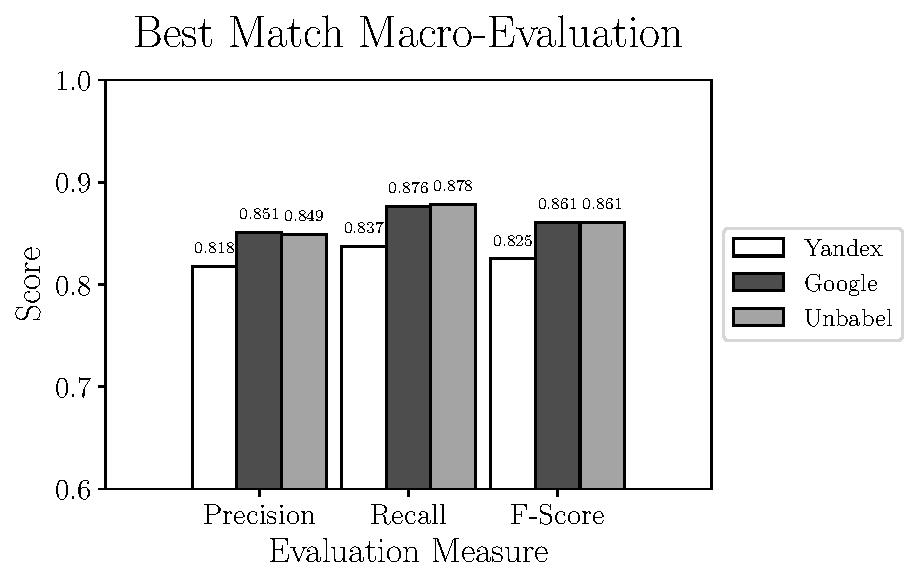
\includegraphics[width=0.9\textwidth]{SupportFiles/plots/best_match_macro_clinical_anatomical_subtrees_plot.pdf}
	\caption{Macro Evaluation of translations being tested, considering just the terms from RadLex \textit{clinical finding} and \textit{anatomical entity} subtrees (Best Match)}
	\label{app:macro_eval_subtrees_best}
\end{figure}


\begin{figure}[ht]
	\centering
	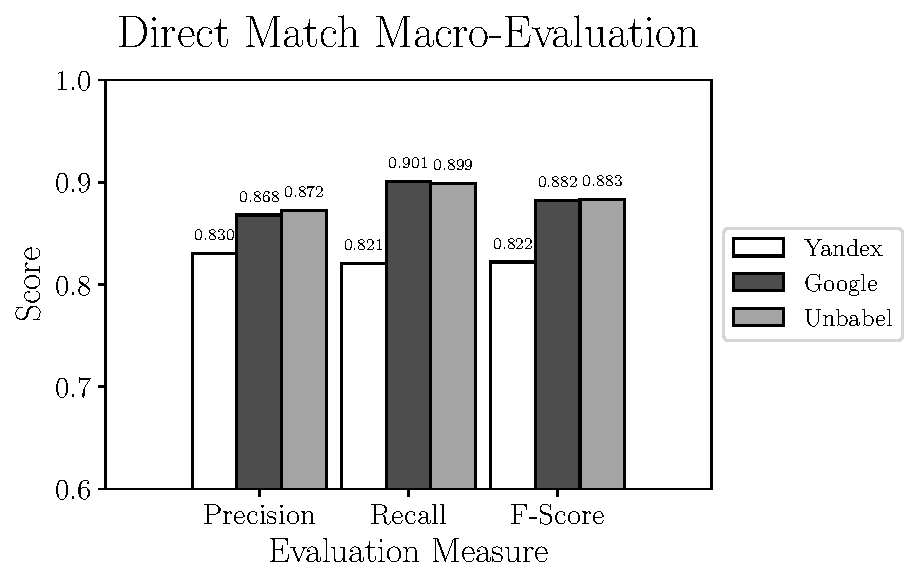
\includegraphics[width=0.9\textwidth]{SupportFiles/plots/direct_match_macro_clinical_anatomical_subtrees_plot.pdf}
	\caption{Macro Evaluation of translations being tested, considering just the terms from RadLex \textit{clinical finding} and \textit{anatomical entity} subtrees (Direct Match)}
	\label{app:macro_eval_subtrees_direct}
\end{figure}

